\section{More Attention Heads in Dormant and Active Phase}\label{sec:more_heads}

In this section, we present two more dormant- and active- phase heads in Llama 2-7B-Base, in \Cref{fig:llama_l16h20,fig:llama_l16h28}, which are more difficult to interpret than Layer 16 Head 25, but go dormant on some inputs and active on others. 

\begin{figure}[h]
    \centering
    \begin{subfigure}[t]{0.475\textwidth}
        \centering 
        \caption{}
        
\includegraphics[width=\linewidth]{Figures/L16H20/github.png}
        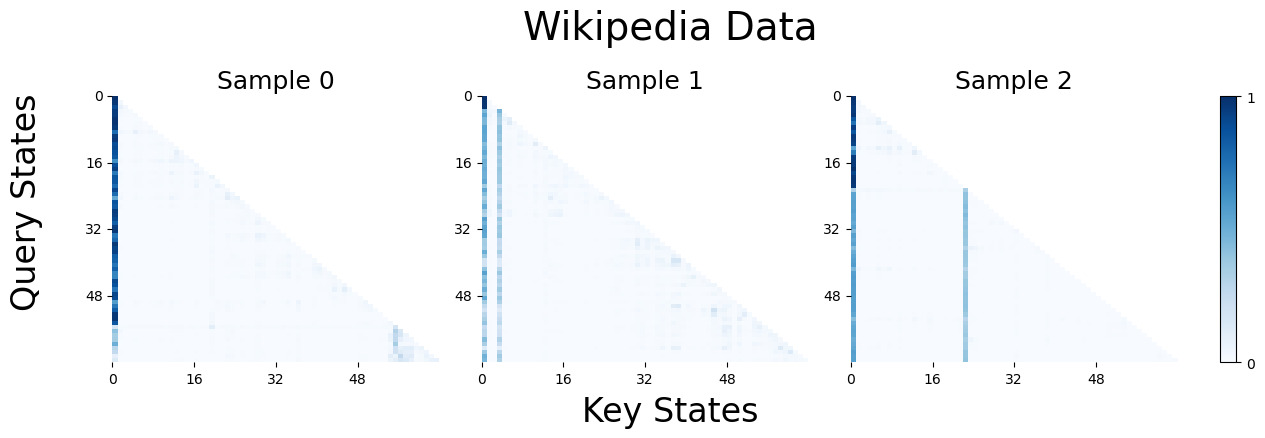
\includegraphics[width=\linewidth]{Figures/L16H20/wikipedia.png}
    \end{subfigure}
    \hfill
    \begin{subfigure}[t]{0.475\textwidth}
        \centering 
        \caption{}
        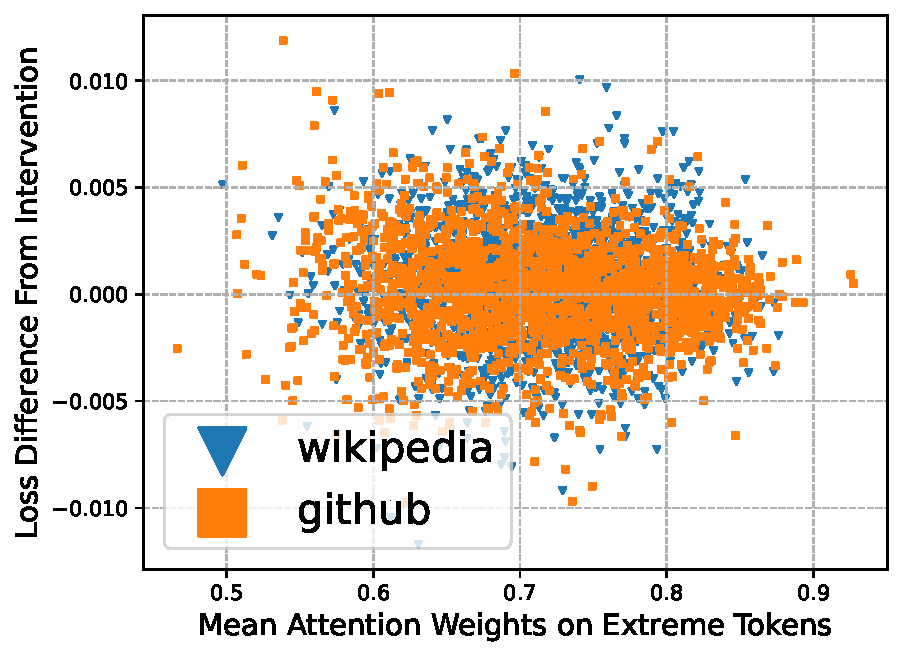
\includegraphics[width=\linewidth]{Figures/L16H20/intervention.pdf}
    \end{subfigure}
    \caption{\small \textbf{Layer 16 Head 20 of Llama 2-7B-Base.}}
    \label{fig:llama_l16h20}
\end{figure}

\begin{figure}
    \centering
    \begin{subfigure}[t]{0.475\textwidth}
        \centering
        \caption{}
        
\includegraphics[width=\linewidth]{Figures/L16H28/github.png}
        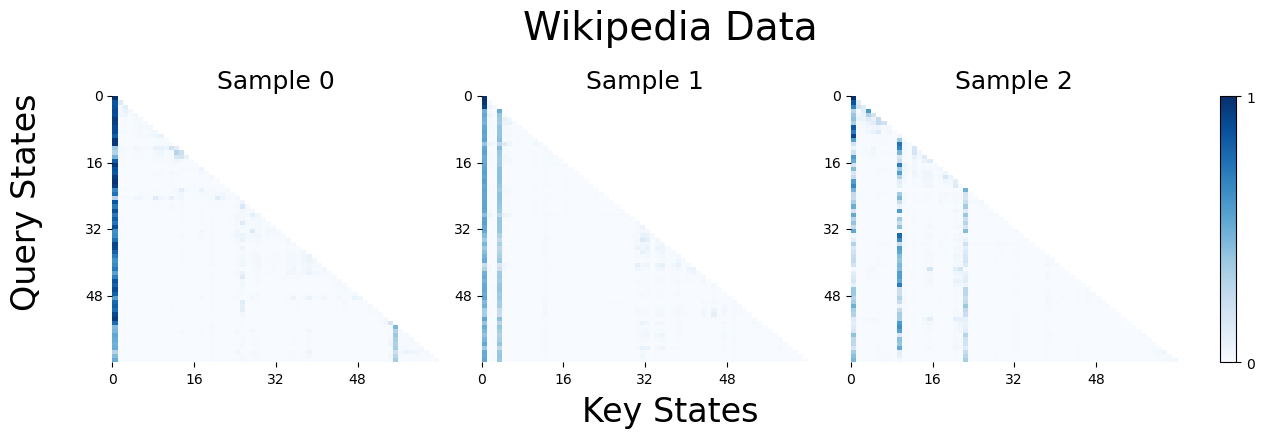
\includegraphics[width=\linewidth]{Figures/L16H28/wikipedia.png}
    \end{subfigure}
    \begin{subfigure}[t]{0.475\textwidth}
        \centering
        \caption{}
        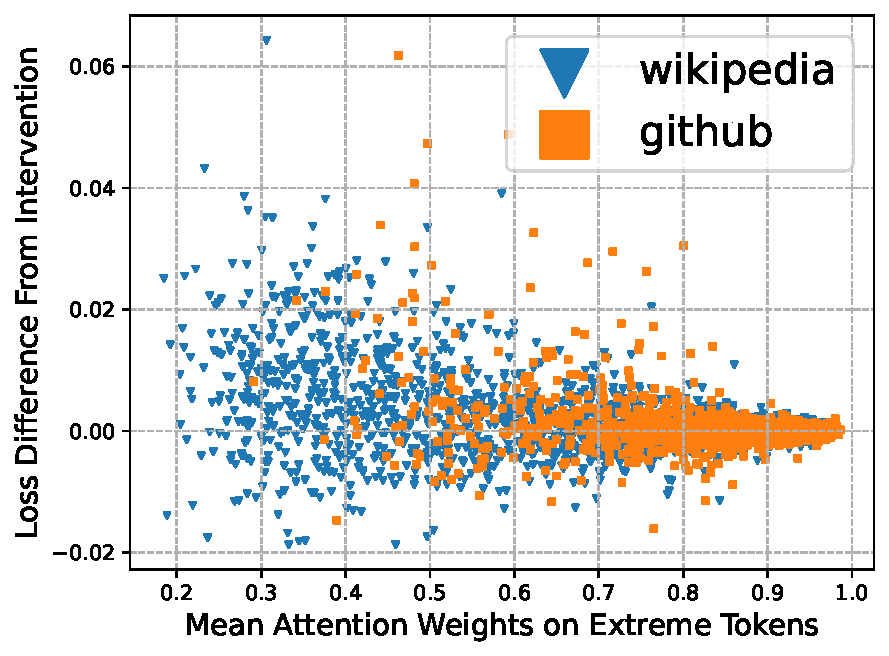
\includegraphics[width=\linewidth]{Figures/L16H28/intervention.pdf}
    \end{subfigure}
    \caption{\small \textbf{Layer 16 Head 28 of Llama 2-7B-Base.}}
    \label{fig:llama_l16h28}
\end{figure}


